% =========================================================================
% Williamson 6 (Rossby-Haurwitz) convergence -- deterministic (--pure).
% No exact solution, so errors are L2 norms of the difference against a
% NUMERICAL reference: finest mesh (ref6) for the spatial study, finest
% timestep (nsteps=2560) for the temporal study. BDM2/DG1 (degree=1),
% coords_degree=2, tmax = 2 days (pre-breakdown of the RH wave).
% Requires \usepackage{booktabs}.
% =========================================================================

% ---------- SPATIAL (vary mesh; reference = ref6; cPG P2 so dt-error negligible) ----------
\begin{table}[htbp]
  \centering
  \begin{tabular}{c c c c c c}
    \toprule
    ref & $h$ (km) & $\|u-u_{\mathrm{ref}}\|_{L^2}$ & rate$_u$
        & $\|D-D_{\mathrm{ref}}\|_{L^2}$ & rate$_D$ \\
    \midrule
    2 & 1785.5 & $1.28\times10^{7}$ & --   & $5.45\times10^{8}$ & --   \\
    3 &  892.8 & $1.75\times10^{6}$ & 2.87 & $1.39\times10^{8}$ & 1.97 \\
    4 &  446.4 & $3.01\times10^{5}$ & 2.54 & $3.47\times10^{7}$ & 2.00 \\
    5 &  223.2 & $5.51\times10^{4}$ & 2.45 & $8.41\times10^{6}$ & 2.04 \\
    \bottomrule
  \end{tabular}
  \caption{Spatial convergence for the Williamson test case~6 (Rossby--Haurwitz wave,
    deterministic), BDM$_2$/DG$_1$ (\texttt{degree}$=1$, \texttt{coords\_degree}$=2$),
    cPG ($P_2$) integrator at $\texttt{nsteps}=256$ ($\Delta t = 675$\,s) so the temporal
    error is negligible, $t = 2$\,days. Errors are $L^2$ norms of the difference against
    the finest-mesh (refinement level~6) numerical reference, with coarse solutions
    cross-mesh interpolated onto it. The depth converges at second order; the velocity is
    super-convergent ($\approx 2.5$). The finest velocity rate ($4\!\to\!5$) is
    reference-limited, since ref~6 is only one level finer than ref~5.}
  \label{tab:w6-spatial}
\end{table}

% ---------- TEMPORAL (fixed mesh ref5; reference = nsteps 2560; cPG P1) ----------
\begin{table}[htbp]
  \centering
  \begin{tabular}{c c c c c c c}
    \toprule
    \texttt{nsteps} & $\Delta t$ (s) & Courant
      & $\|u-u_{\mathrm{ref}}\|_{L^2}$ & rate$_u$
      & $\|D-D_{\mathrm{ref}}\|_{L^2}$ & rate$_D$ \\
    \midrule
     80 & 2160 & 0.48 & $9.46\times10^{6}$ & --   & $1.61\times10^{8}$ & --   \\
    160 & 1080 & 0.24 & $4.70\times10^{6}$ & 1.01 & $1.24\times10^{8}$ & 0.38 \\
    320 &  540 & 0.12 & $1.28\times10^{6}$ & 1.88 & $5.55\times10^{7}$ & 1.16 \\
    640 &  270 & 0.06 & $3.42\times10^{5}$ & 1.90 & $1.34\times10^{7}$ & 2.05 \\
    \bottomrule
  \end{tabular}
  \caption{Temporal convergence for the Williamson test case~6 (Rossby--Haurwitz wave,
    deterministic) on a fixed mesh (refinement level~5, BDM$_2$/DG$_1$) with the cPG
    ($P_1$) integrator, $t = 2$\,days. Errors are $L^2$ norms of the difference against a
    fine-timestep numerical reference ($\texttt{nsteps}=2560$, $\Delta t = 67.5$\,s) on
    the same mesh. Both fields converge at second order, approached from below: at the
    coarsest $\Delta t$ ($2160$\,s) the Rossby--Haurwitz dynamics are not yet in the
    asymptotic regime, so the rates climb to $\sim 2$ as $\Delta t$ is refined
    ($\texttt{nsteps}=320\!\to\!640$: $1.90$ for $u$, $2.05$ for $D$).}
  \label{tab:w6-temporal}
\end{table}

% ---------- Diagnostic figures (require \usepackage{graphicx}) ----------
% Upload w6_div_norms.png and w6_energy_errors.png to the Overleaf project.
\begin{figure}[htbp]
  \centering
  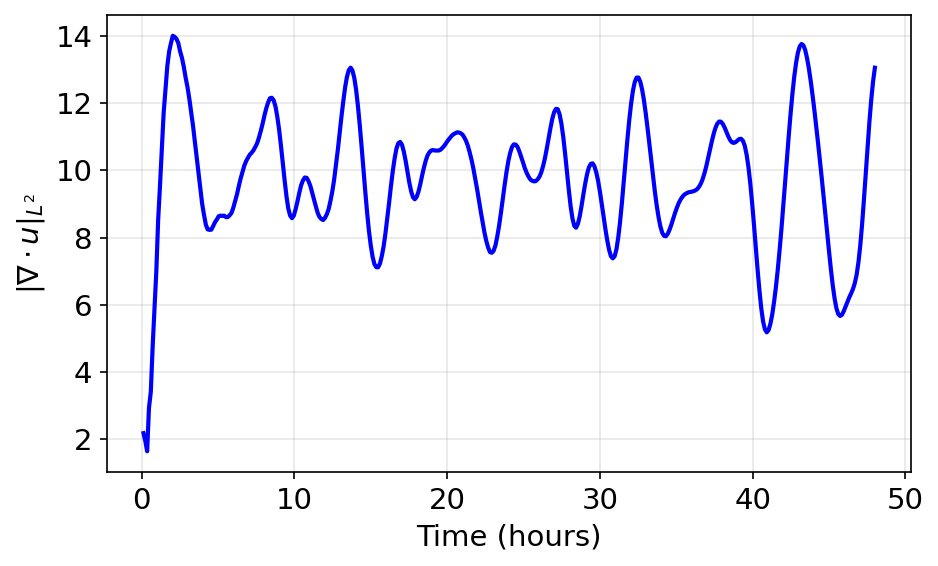
\includegraphics[width=0.8\textwidth]{w6_div_norms.png}
  \caption{Velocity divergence $\|\nabla\cdot u\|_{L^2}$ versus time for the Williamson
    test case~6 (Rossby--Haurwitz wave, deterministic), BDM$_2$/DG$_1$ on refinement
    level~5 with $\Delta t = 67.5$\,s. The flow, initialised as $u=\nabla^{\perp}\psi$
    (exactly divergence-free), develops only a small bounded divergence
    ($\|\nabla\cdot u\|/\|u\| \sim 10^{-7}$) that oscillates with the wave dynamics.}
  \label{fig:w6-div}
\end{figure}

\begin{figure}[htbp]
  \centering
  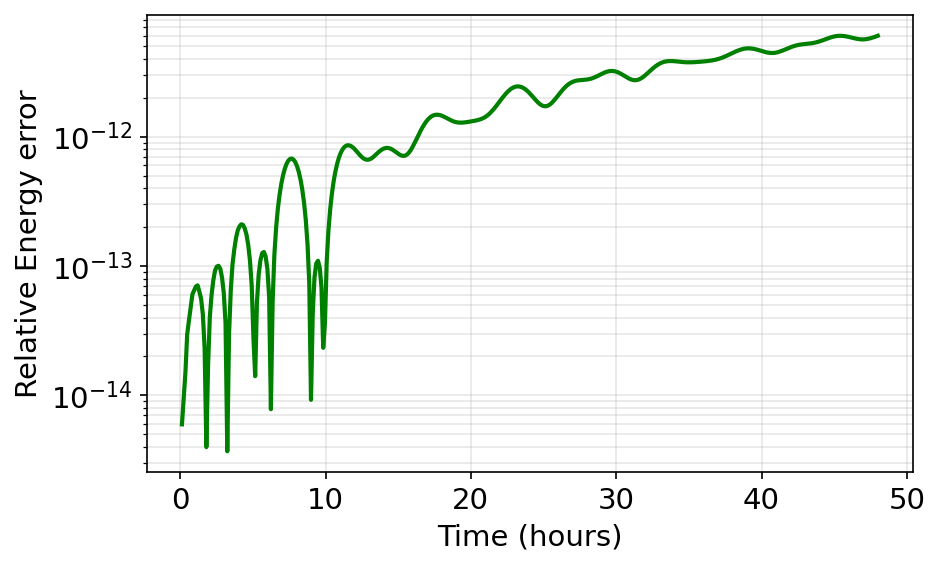
\includegraphics[width=0.8\textwidth]{w6_energy_errors.png}
  \caption{Relative energy drift $|(E-E_0)/E_0|$ versus time for the Williamson test
    case~6 (Rossby--Haurwitz wave, deterministic), BDM$_2$/DG$_1$ on refinement level~5
    with $\Delta t = 67.5$\,s. The energy is conserved to solver/round-off precision
    ($\lesssim 3\times10^{-11}$) over two days, confirming the energy-conserving property
    of the fully discrete scheme for this test case.}
  \label{fig:w6-energy}
\end{figure}
